

\chapter{Implementation}

\label{Implementation}

\section{Architecture}

TODO: architecture details, sample of spring application context,
description of a problem domain and fitness function

\lstinputlisting{test-context.xml}

\section{Implementation in Java}
clean structure, good test coverage, 
modular architercture, extensible,

\subsection{Technologies}
\begin{itemize}
  \item Spring \cite{spring} - application framework
  \item Maven \cite{maven} - project management and build automation
  \item Mockito \cite{mockito} - testing framework 
  \item JAMA \cite{jama} - linear algebra package
\end{itemize}
Spring, Maven, JUnit, Mockito, JAMA, TDD approach

\subsection{Diagrams}
class diagrams, sequence diagrams

Below you may find class diagrams for each of the module implemented in our
framework. It shows a general overview of the structure of a system: used
classes, their attributes, operations and the relationships between the classes.


\begin{figure}
  \centering
  \fbox{
    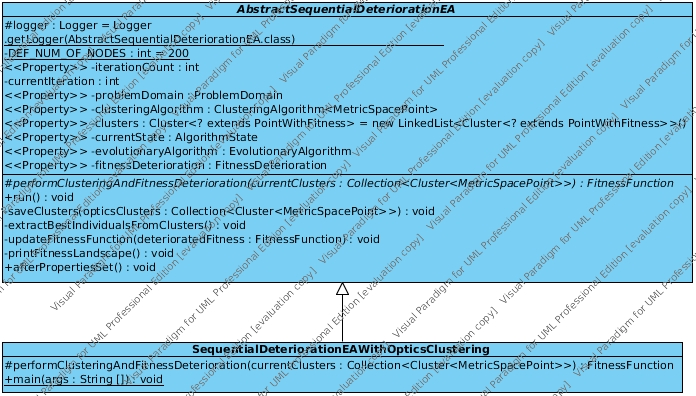
\includegraphics[scale=0.5]{ClassDiagrams/algorithm.jpg}
  }
  \caption{Main algorithm package}
  \label{alg}
\end{figure}

\begin{figure}
  \centering
  \fbox{
    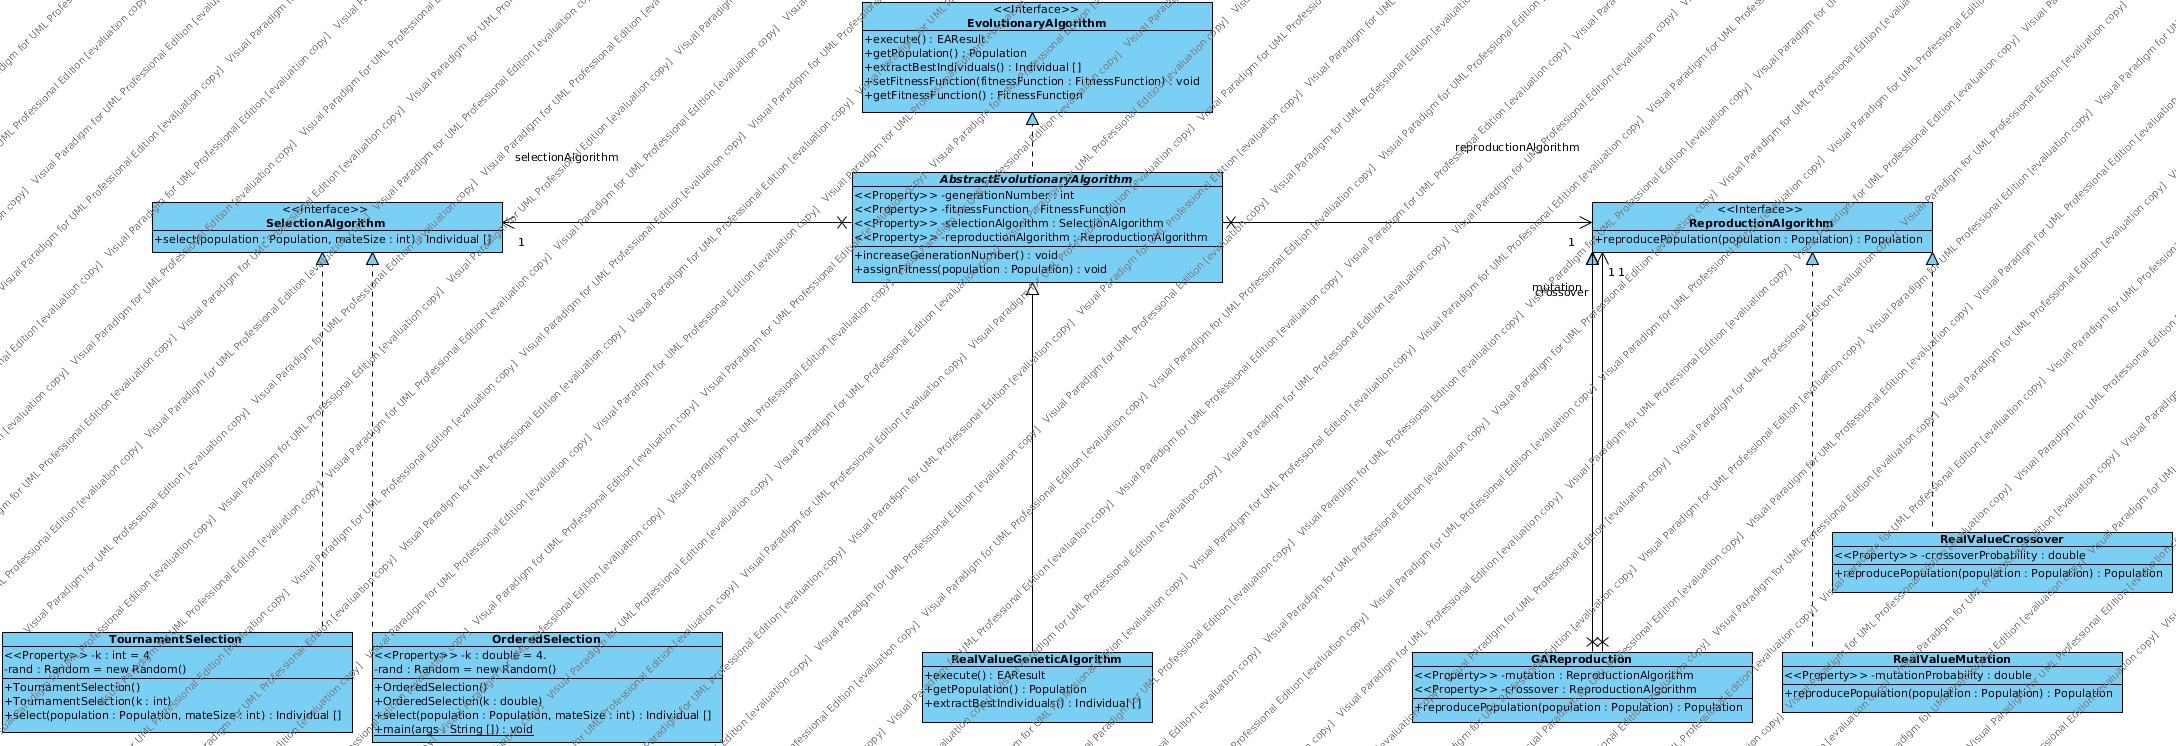
\includegraphics[scale=0.3, angle=90]{ClassDiagrams/EA.jpg}
  }
  \caption{Evolutionary algorithms package}
  \label{ea}
\end{figure}

\begin{figure}
  \centering
  \fbox{
    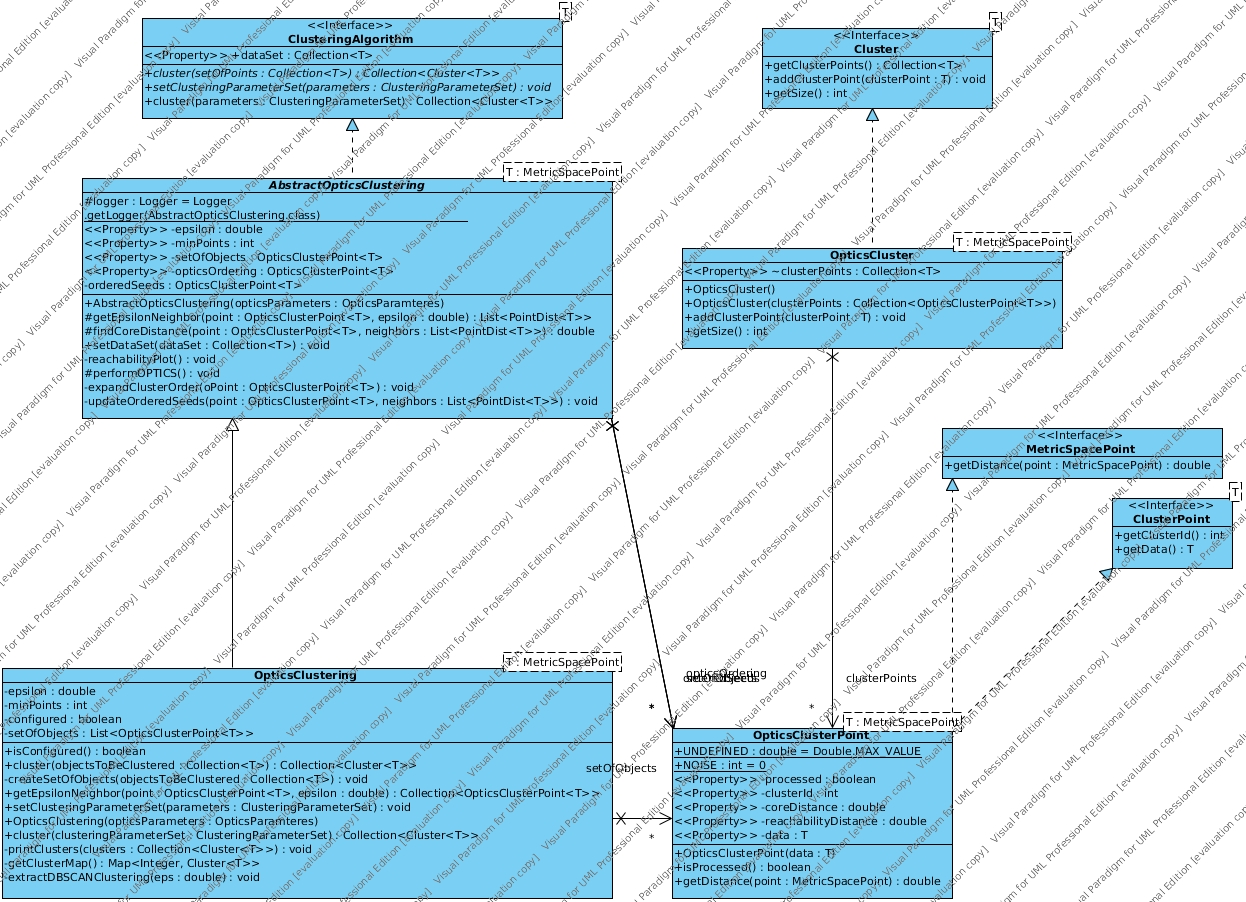
\includegraphics[scale=0.3, angle=90]{ClassDiagrams/clustering.jpg}
  }
  \caption{Clustering package}
  \label{optics}
\end{figure}

\begin{figure}
  \centering
  \fbox{
    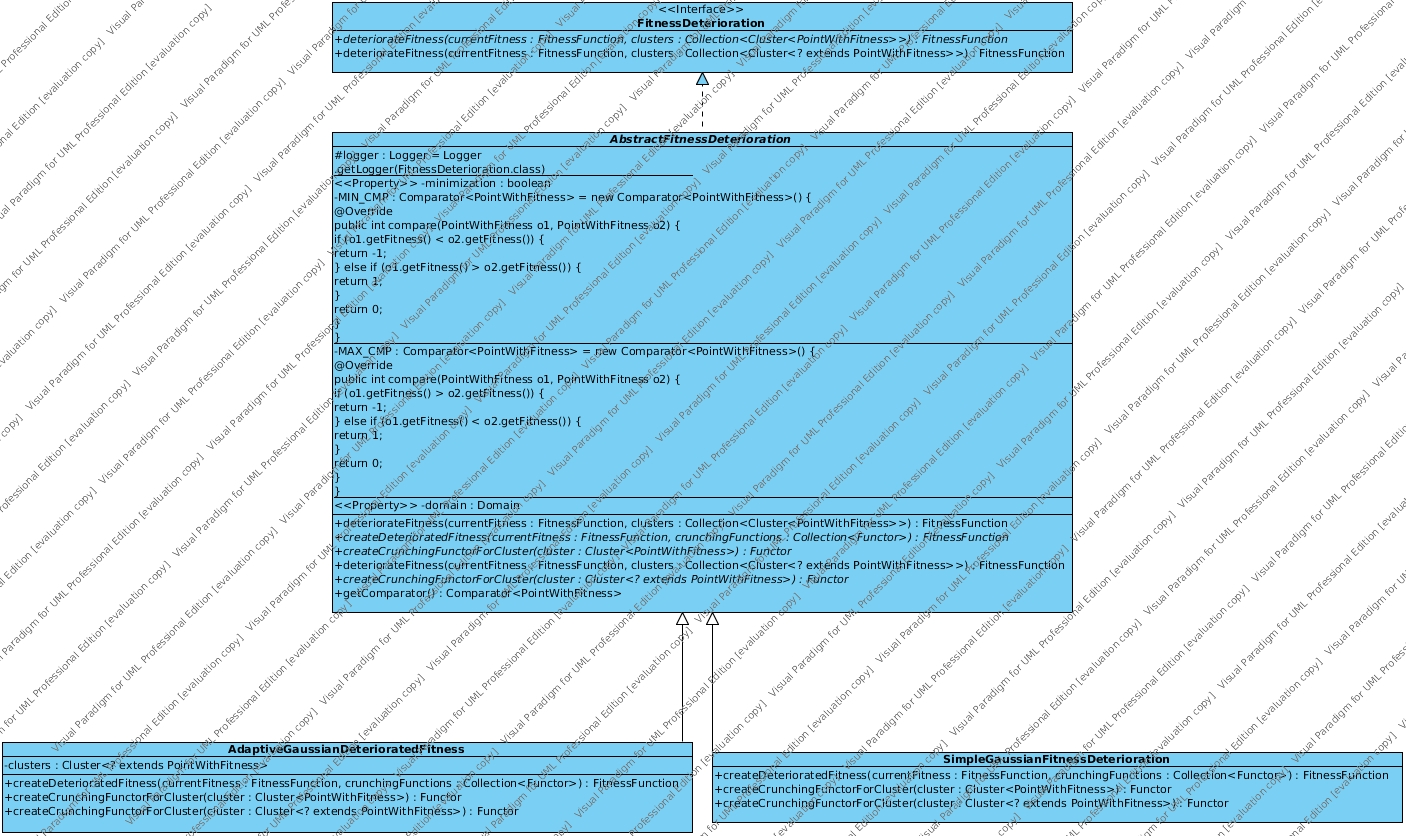
\includegraphics[scale=0.3, angle=90]{ClassDiagrams/deterioration.jpg}
  }
  \caption{Fitness deterioration package}
  \label{fitdet}
\end{figure}

\begin{figure}
  \centering
  \fbox{
    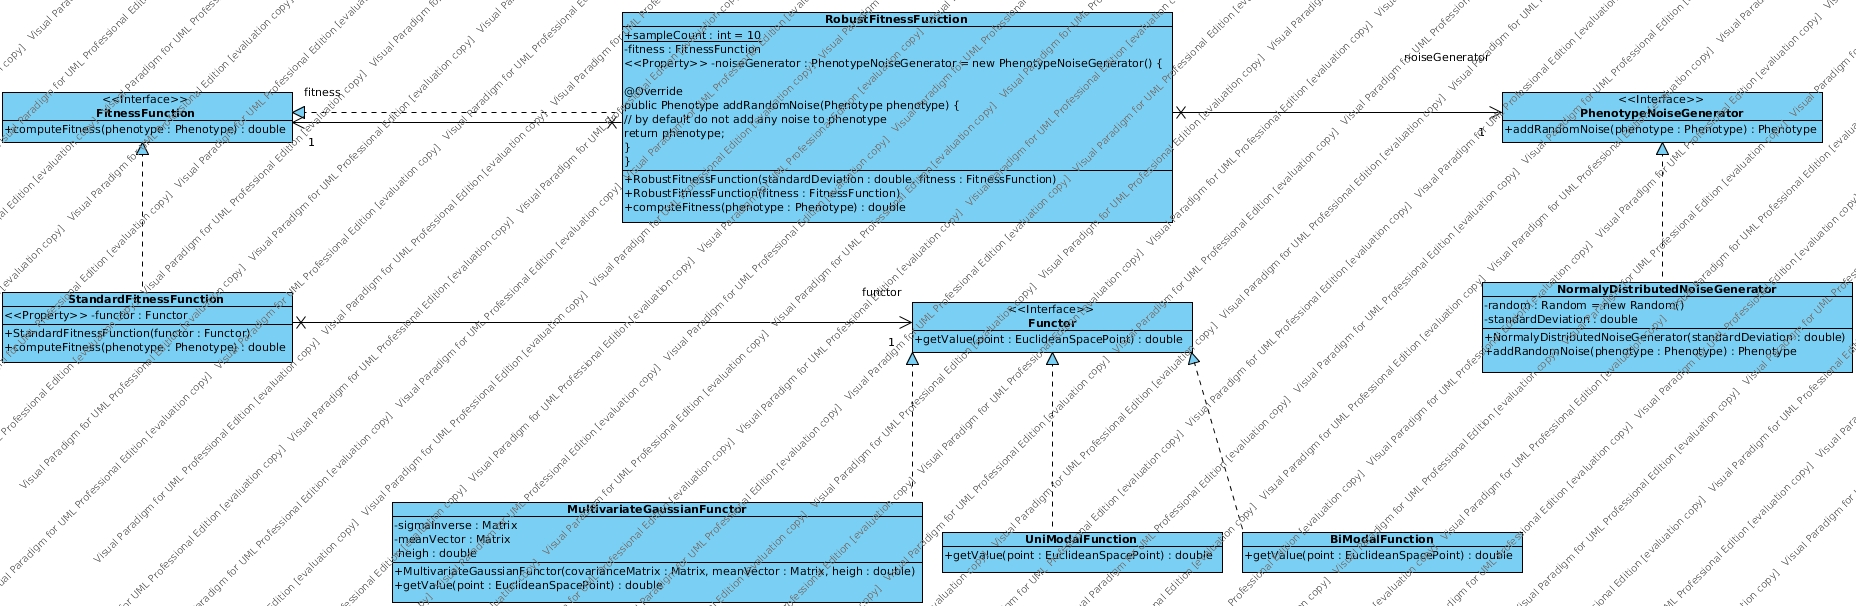
\includegraphics[scale=0.3, angle=90]{ClassDiagrams/fitness.jpg}
  }
  \caption{Fitness and functors package}
  \label{ea}
\end{figure}

\begin{figure}
  \centering
  \fbox{
    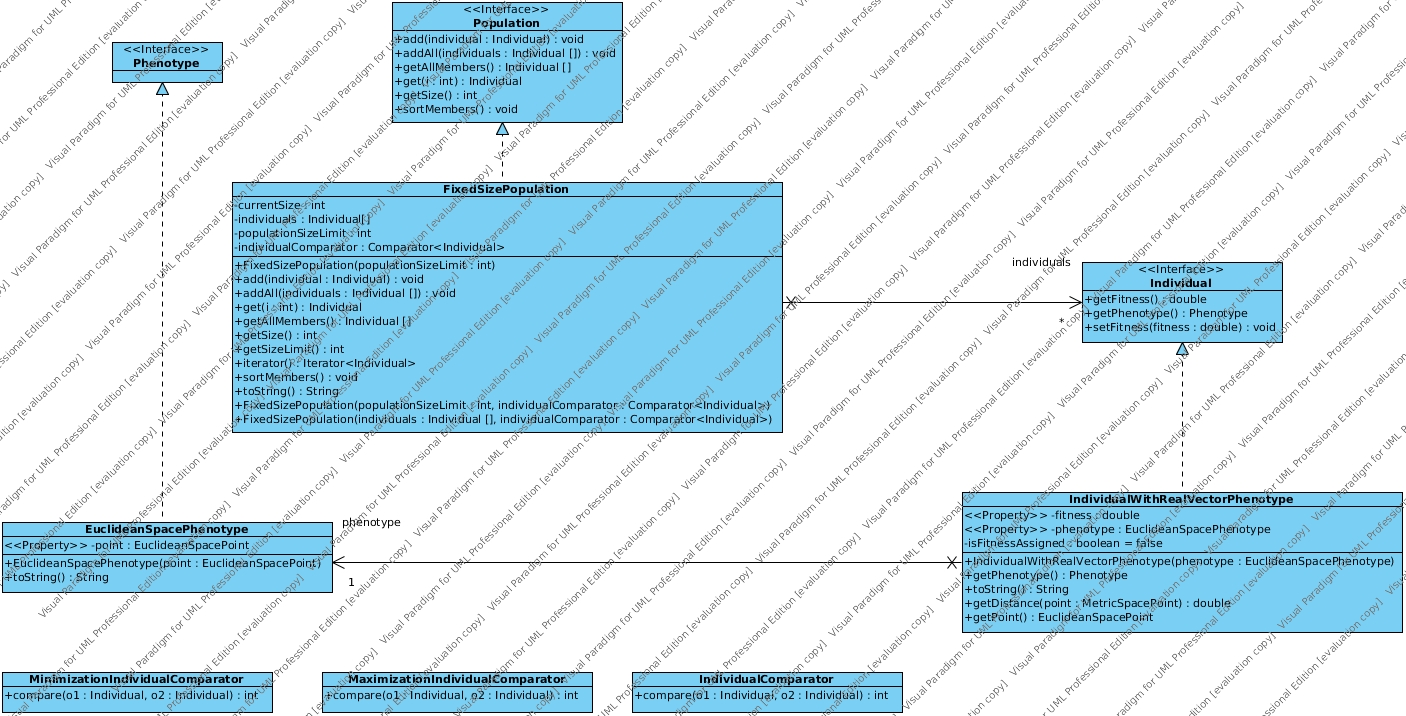
\includegraphics[scale=0.3, angle=90]{ClassDiagrams/population.jpg}
  }
  \caption{Population package}
  \label{ea}
\end{figure}